\documentclass{article}

\usepackage{graphicx}
\usepackage{tikz}
\usepackage{tikzsymbols}
\usetikzlibrary{calc,patterns,shapes.geometric}
\pagestyle{empty}
\usepackage[margin=0pt]{geometry}
\geometry{papersize={14in,12in}}

\def\centerarc[#1](#2)(#3:#4:#5){\draw[#1] ($(#2)+({#5*cos(#3)},{#5*sin(#3)})$) arc (#3:#4:#5);}

\begin{document}
	\begin{figure}
		\centering
		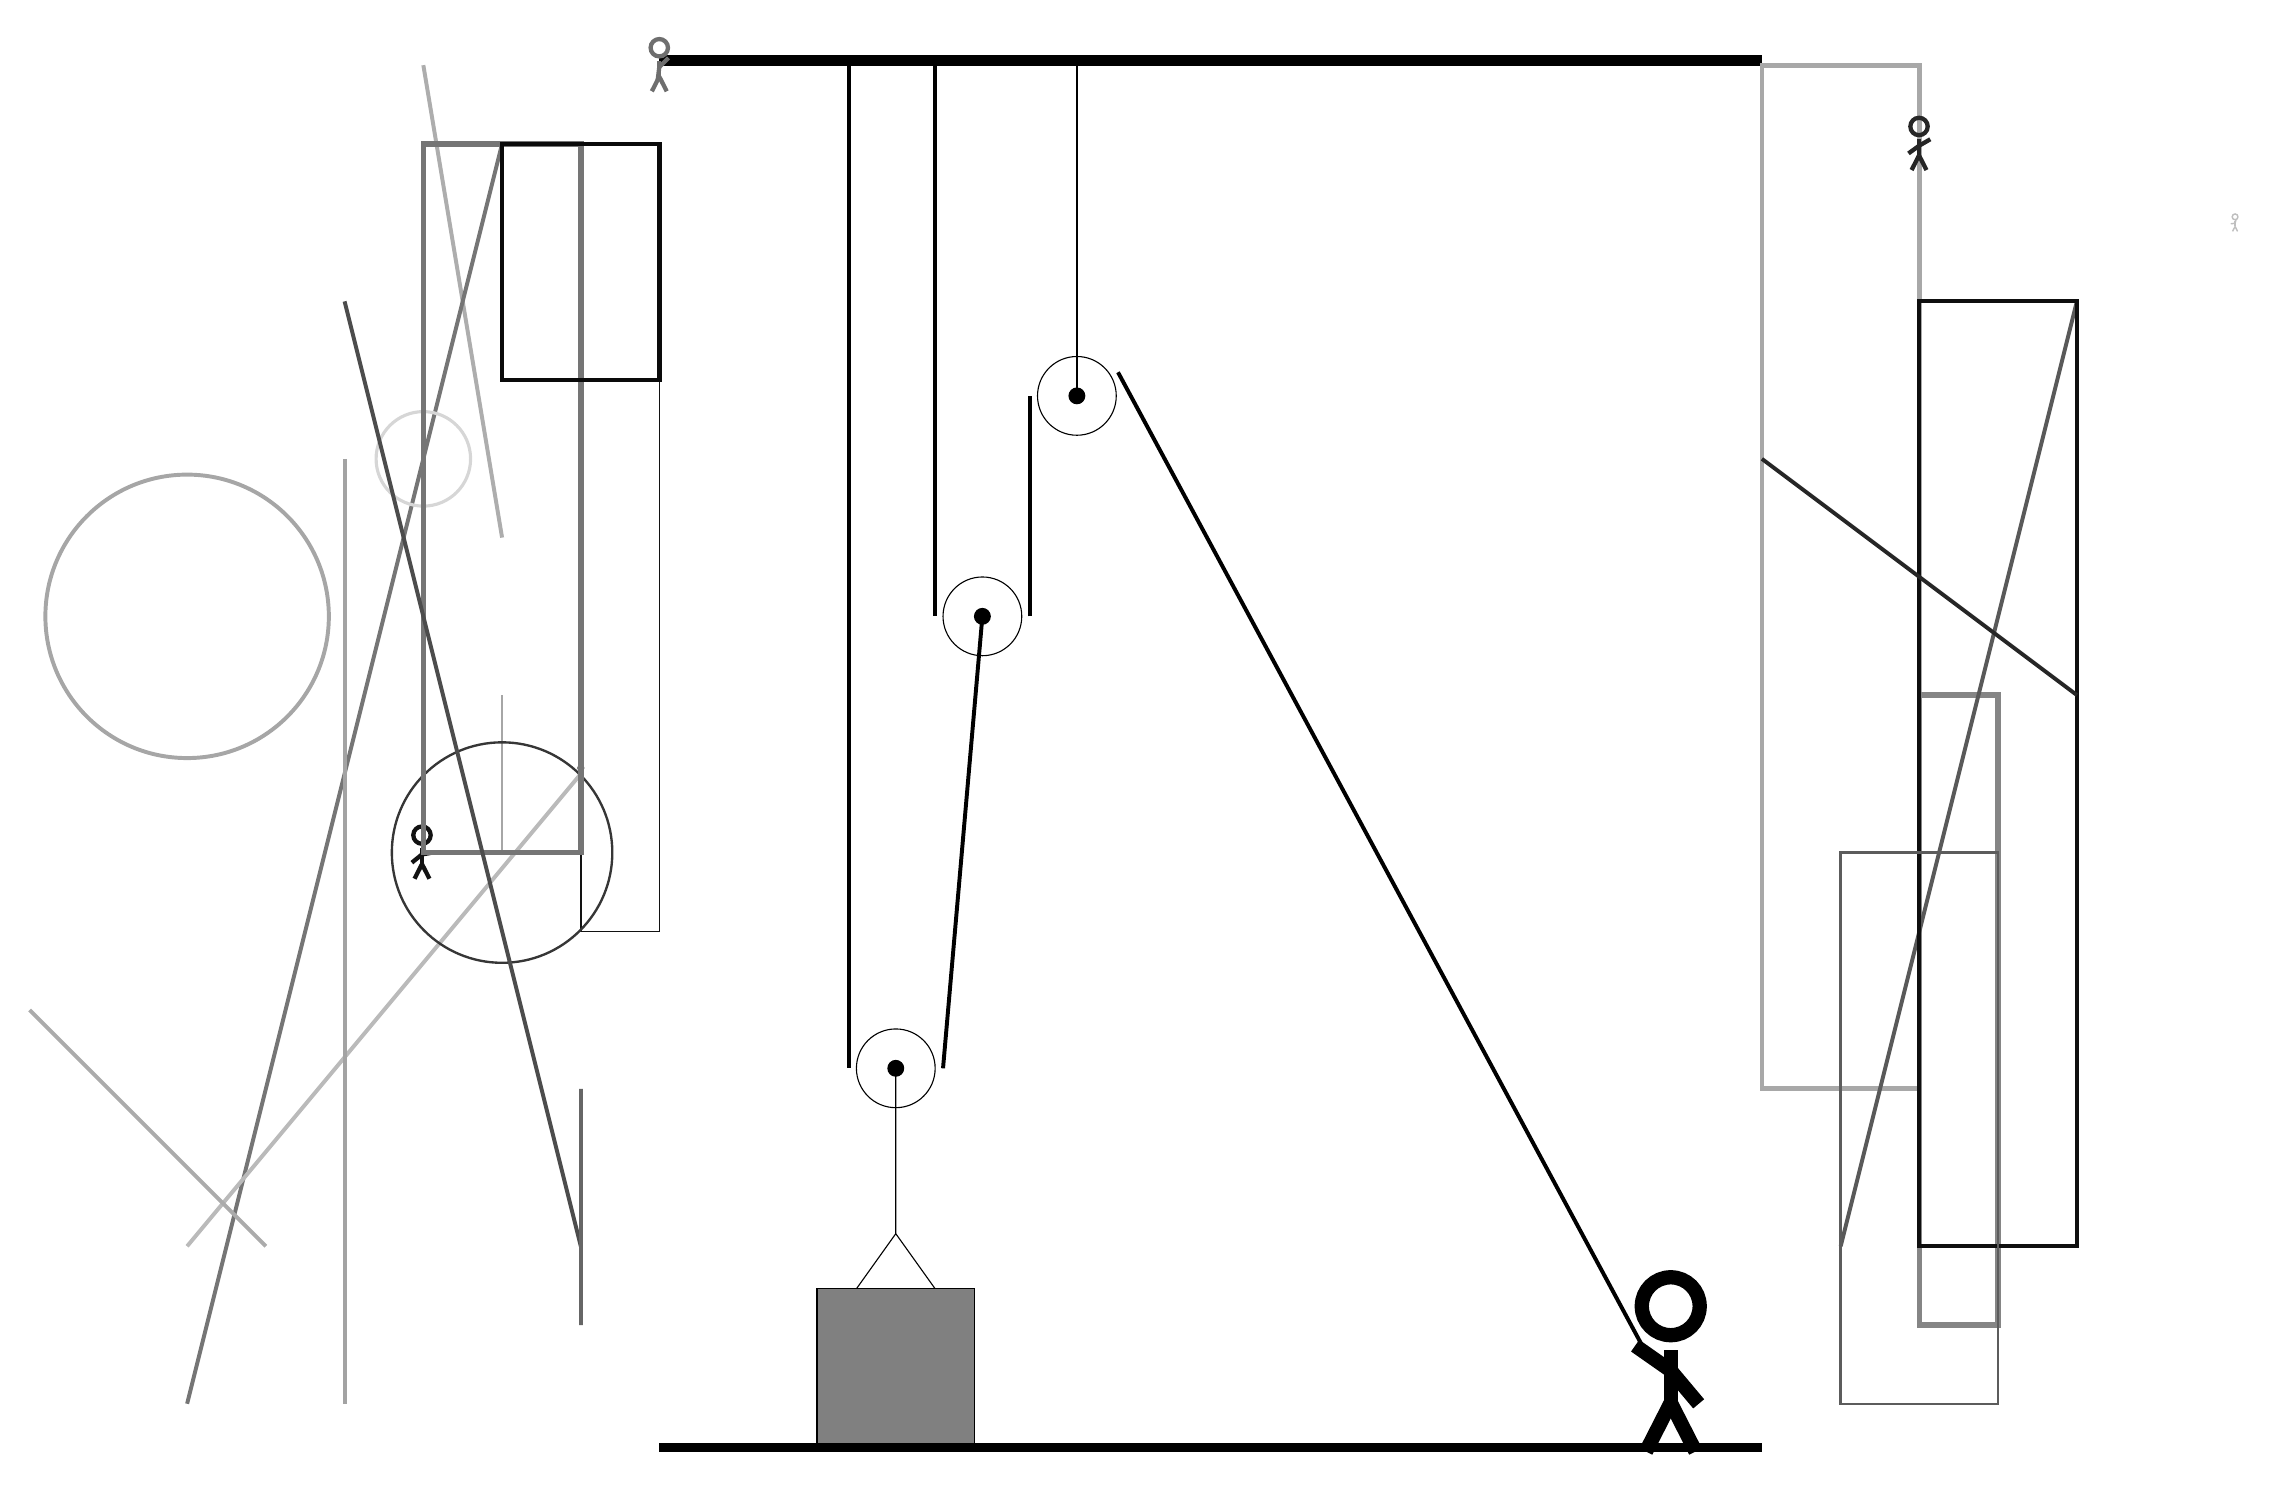
\begin{tikzpicture}
			%%%%% START %%%%%
			
			\draw[fill=black] (-2, 14) rectangle (12, 14.125);
			
			\draw (1, 1.26) circle (0.5);
			\draw[fill=black] (1, 1.26) circle (0.1);
			
			\draw (2.1, 7.0) circle (0.5);
			\draw[fill=black] (2.1, 7.0) circle (0.1);
			
			\draw (3.3, 9.8) circle (0.5);
			\draw[fill=black] (3.3, 9.8) circle (0.1);
			\draw[thick] (3.3, 9.8) -- (3.3, 14);
			
			\draw (1, 1.26) -- (1, -0.84) -- (0.5, -1.54) -- (1.5, -1.54) -- (1, -0.84);
			\draw[fill=black!50] (0, -1.54) rectangle (2, -3.54);
			
			\draw[line width=0.5mm, color=black!32](-5, 14) -- (-4, 8);
			
			\draw [line width=0.5mm, color=black!35](-8, 7) circle (1.8);
			\draw[line width=0.6mm, color=black!34] (14, 14) rectangle (12, 1);
			\draw[line width=0.5mm, color=black!54](-4, 13) -- (-8, -3);
			
			\draw[line width=0.2mm, color=black!93] (-3, 3) rectangle (-2, 13);
			\draw[line width=0.7mm, color=black!48] (14, -2) rectangle (15, 6);
			
			\node[line width=0.7mm, color=black!93] at (-5, 4) {\Strichmaxerl[3][39][10]};
			\draw[line width=0.5mm, color=black!27](-3, 5) -- (-8, -1);
			\node[line width=0.5mm, color=black!66] at (-3, 5) {\Strichmaxerl[1][74][63]};
			
			\node[line width=0.2mm, color=black!85] at (14, 13) {\Strichmaxerl[3][36][30]};
			\draw[line width=0.5mm, color=black!65](16, 11) -- (13, -1);
			
			\draw[line width=0.2mm, color=black!35] (-4, 6) rectangle (-4, 4);
			\draw[line width=0.5mm, color=black!33](-7, -1) -- (-10, 2);
			
			\draw [line width=0.4mm, color=black!16](-5, 9) circle (0.6);
			\draw [line width=0.3mm, color=black!79](-4, 4) circle (1.4);
			\draw[line width=0.7mm, color=black!54] (-3, 13) rectangle (-5, 4);
			
			\draw[line width=0.5mm, color=black!70](-3, -1) -- (-6, 11);
			\draw[line width=0.5mm, color=black!36](-6, 9) -- (-6, -3);
			\draw[line width=0.6mm, color=black!96] (-4, 13) rectangle (-2, 10);
			
			\draw[line width=0.5mm, color=black!94] (14, -1) rectangle (16, 11);
			\draw[line width=0.3mm, color=black!64] (13, 4) rectangle (15, -3);
			\draw[line width=0.5mm, color=black!60] (-3, 1) rectangle (-3, -2);
			
			\node[line width=0.5mm, color=black!25] at (18, 12) {\Strichmaxerl[1][7][76]};
			\node[line width=0.7mm, color=black!57] at (-2, 14) {\Strichmaxerl[3][83][45]};
			\draw[line width=0.5mm, color=black!85](16, 6) -- (12, 9);
			
			\draw[line width=0.5mm] (0.4, 14) -- (0.4, 1.26);
			\centerarc[line width=0.5mm](1, 1.26)(180:360:0.6);
			\draw[line width=0.5mm](1.6, 1.26) -- (2.1, 7.0);
			\draw[line width=0.5mm] (1.5, 14) -- (1.5, 7.0);
			\centerarc[line width=0.5mm](2.1, 7.0)(180:360:0.6);
			\draw[line width=0.5mm](2.7, 7.0) -- (2.7, 9.8);
			\centerarc[line width=0.5mm](3.3, 9.8)(30:180:0.6);
			\draw[line width=0.5mm] (3.822, 10.1) -- (10.5, -2.3);
			
			\node at (10.8, -2.5) {\Strichmaxerl[10][-35][-50]};
			
			\draw[fill=black] (-2, -3.5) rectangle (12, -3.6);
			
			%%%%% END %%%%%
		\end{tikzpicture}
	\end{figure}	
\end{document}